%%
%% Author: Dario Chinelli
%% begin 2019-12-04
%% last mod 2022-02-02
%%

% Preamble
\documentclass[class=article, crop=false]{standalone}

% Packages
\usepackage[subpreambles=true]{standalone}
\usepackage{import}
\usepackage{graphicx}
\usepackage{amsmath}

% Document
\begin{document}
% Approximation of path integrals: 3D histogram documentation here
The discrete path integral delineated with the models above is capable of great predictions.
But this structures are hard to represents, moreover the models that includes more than 3 indexes is impossible to represents.
To solve this situation here is used a 3D-histogram.
As histogram this plot express the statistic relevance of a certain data that occurred in dataset.
The 3D space dimensions are: the $x$ direction, the $y$ direction and the $time$ dimension that goes upward.
A 2D surface here represents points in the space-time that have the same occurrence, it's also called \emph{isosurface}.

\subsection{3D comparison between real data and simulations}
In this work are considered the \textbf{real data} and the four simulations: \textbf{simD2Q9}, \textbf{simD2Q9Q9}, \textbf{simTD2Q9}, \textbf{simTD2Q9Q9}.
Those simulations are generated starting from respectively the four models: \textbf{D2Q9}, \textbf{D2Q9Q9}, \textbf{TD2Q9}, \textbf{TD2Q9Q9}.

In the figures below are showed the isosurfaces colored by type:
\begin{itemize}
\item BLACK: RealData;
\item LIGHT-BLUE: Simulation D2Q9;
\item PURPLE: Simulation D2Q9Q9;
\item GREEN: Simulation TD2Q9;
\item RED: Simulation TD2Q9Q9.
\end{itemize}

\newpage

\FloatBarrier
\subsection{Plot of the RealData}

\begin{figure}[ht]
\begin{minipage}[c]{0.5\linewidth}
\centering
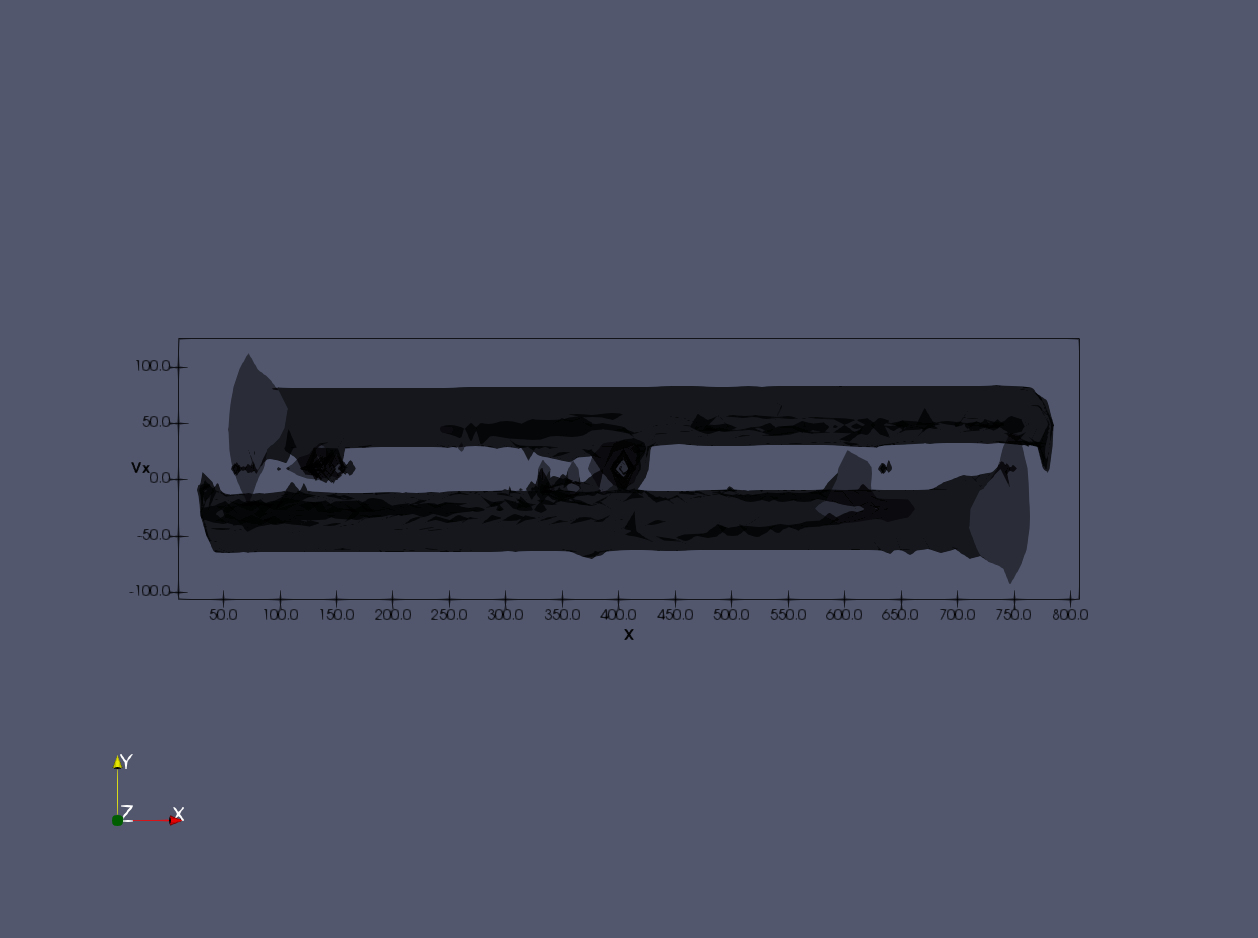
\includegraphics[ width=0.9\textwidth]{fig/3d-hist/trainf10_X_Vx_RealData}
\captionsetup{width=.8\linewidth}
\caption{CAPTION ONE}
\label{fig:comp_RD_1}
\end{minipage}
\begin{minipage}[c]{0.5\linewidth}
\centering
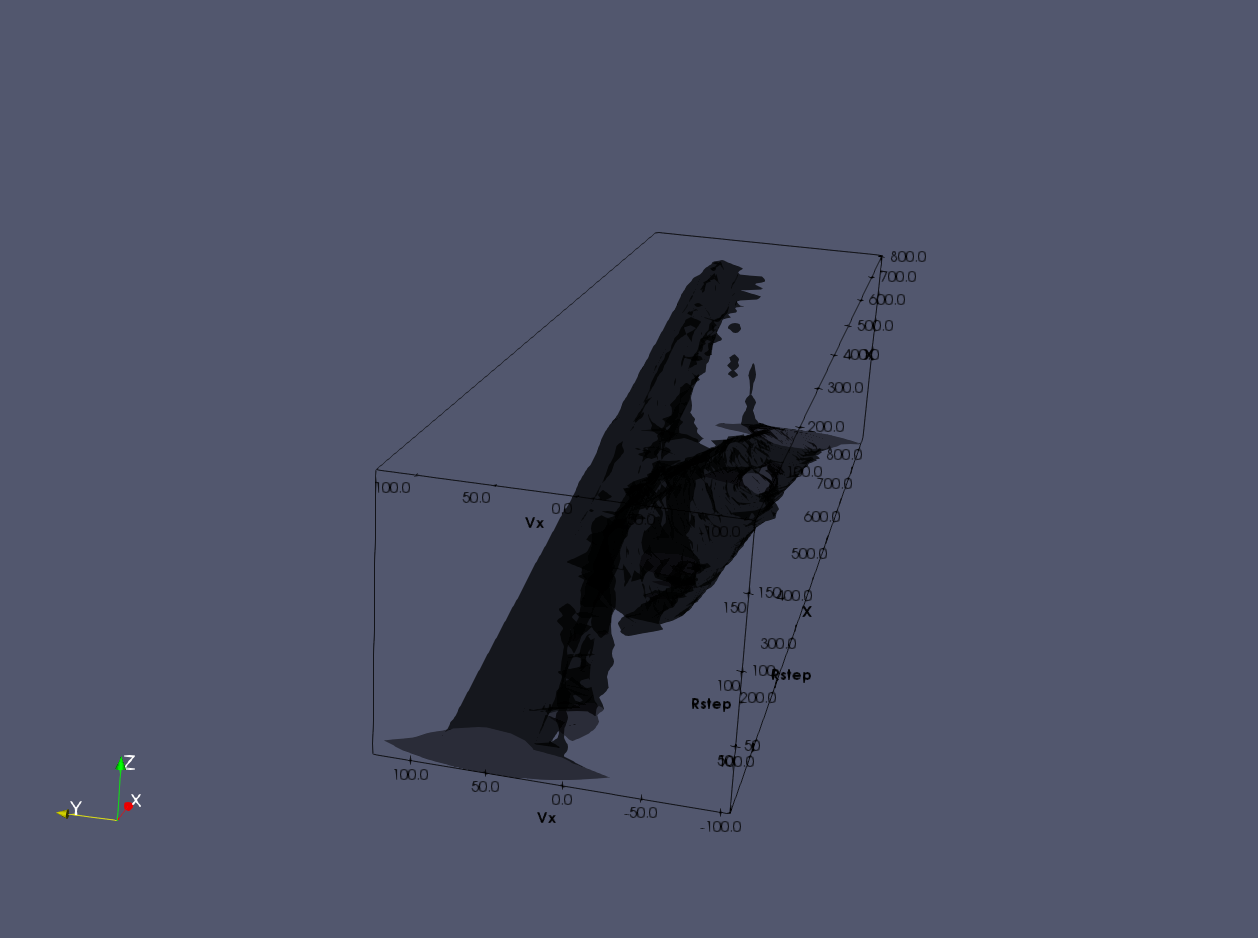
\includegraphics[ width=0.9\textwidth]{fig/3d-hist/trainf10_X_Vx_RealData-2}
\captionsetup{width=.8\linewidth}
\caption{CAPTION TWO}
\label{fig:comp_RD_2}
\end{minipage}
\end{figure}


\FloatBarrier
\subsection{Comparison between RealData and Simulation with D2Q9 model}

\begin{figure}[ht]
\begin{minipage}[c]{0.5\linewidth}
\centering
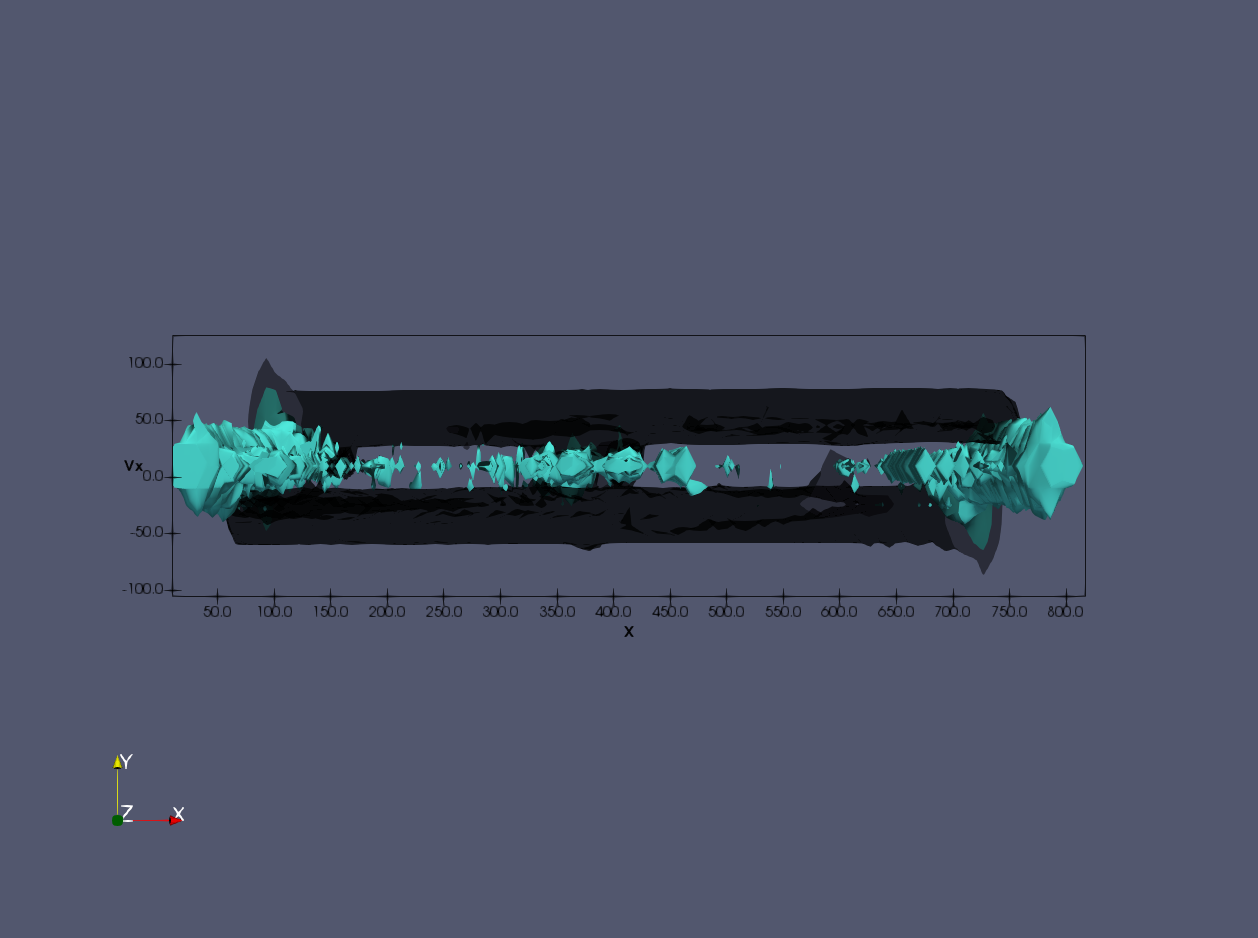
\includegraphics[ width=0.9\textwidth]{fig/3d-hist/trainf10_X_Vx_RealData_and_simD2Q9}
\captionsetup{width=.8\linewidth}
\caption{CAPTION ONE}
\label{fig:comp_RD_D2Q9_1}
\end{minipage}
\begin{minipage}[c]{0.5\linewidth}
\centering
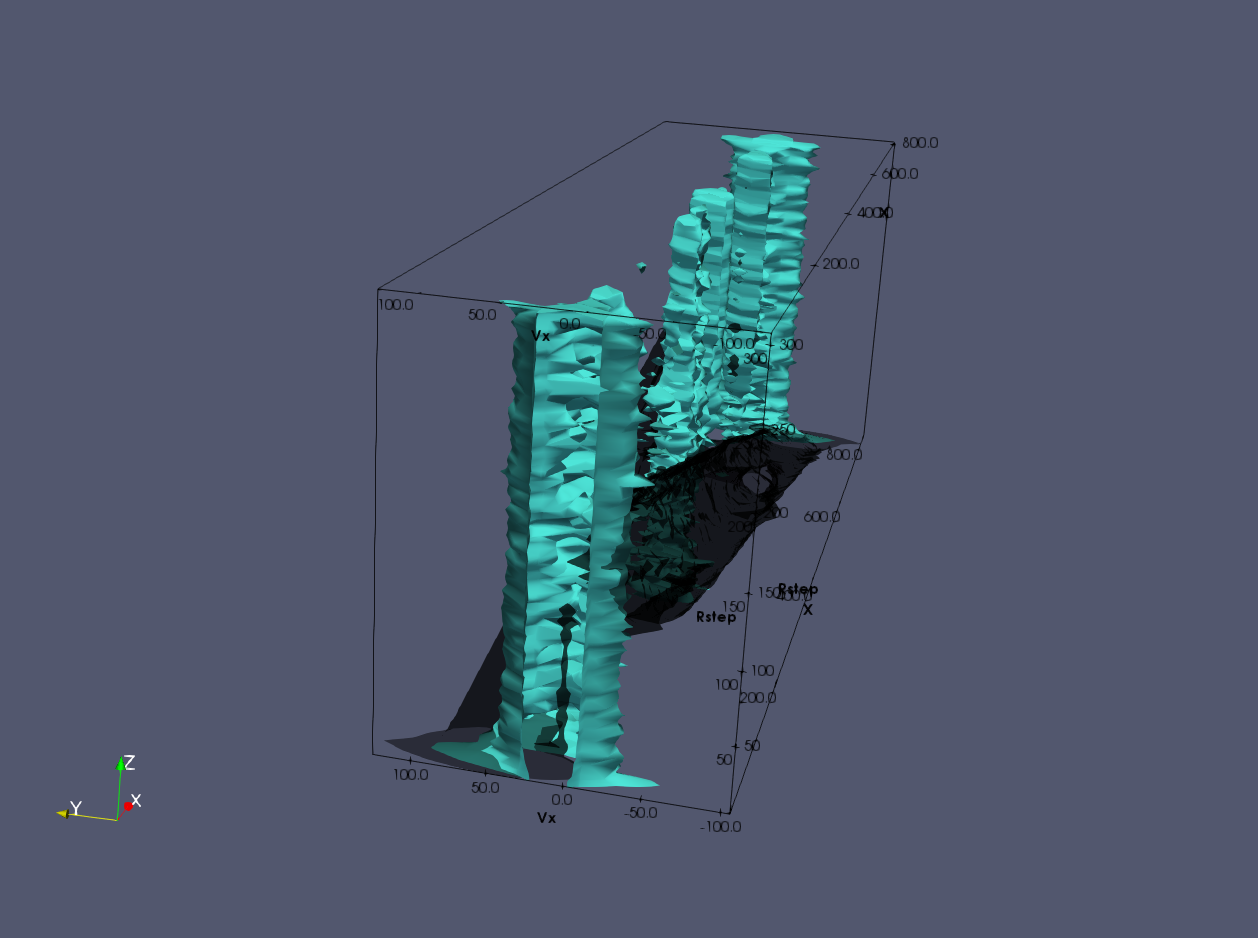
\includegraphics[ width=0.9\textwidth]{fig/3d-hist/trainf10_X_Vx_RealData_and_simD2Q9-2}
\captionsetup{width=.8\linewidth}
\caption{CAPTION TWO}
\label{fig:comp_RD_D2Q9_2}
\end{minipage}
\end{figure}


\FloatBarrier
\subsection{Comparison between RealData and Simulation with D2Q9Q9 model}

\begin{figure}[ht]
\begin{minipage}[c]{0.5\linewidth}
\centering
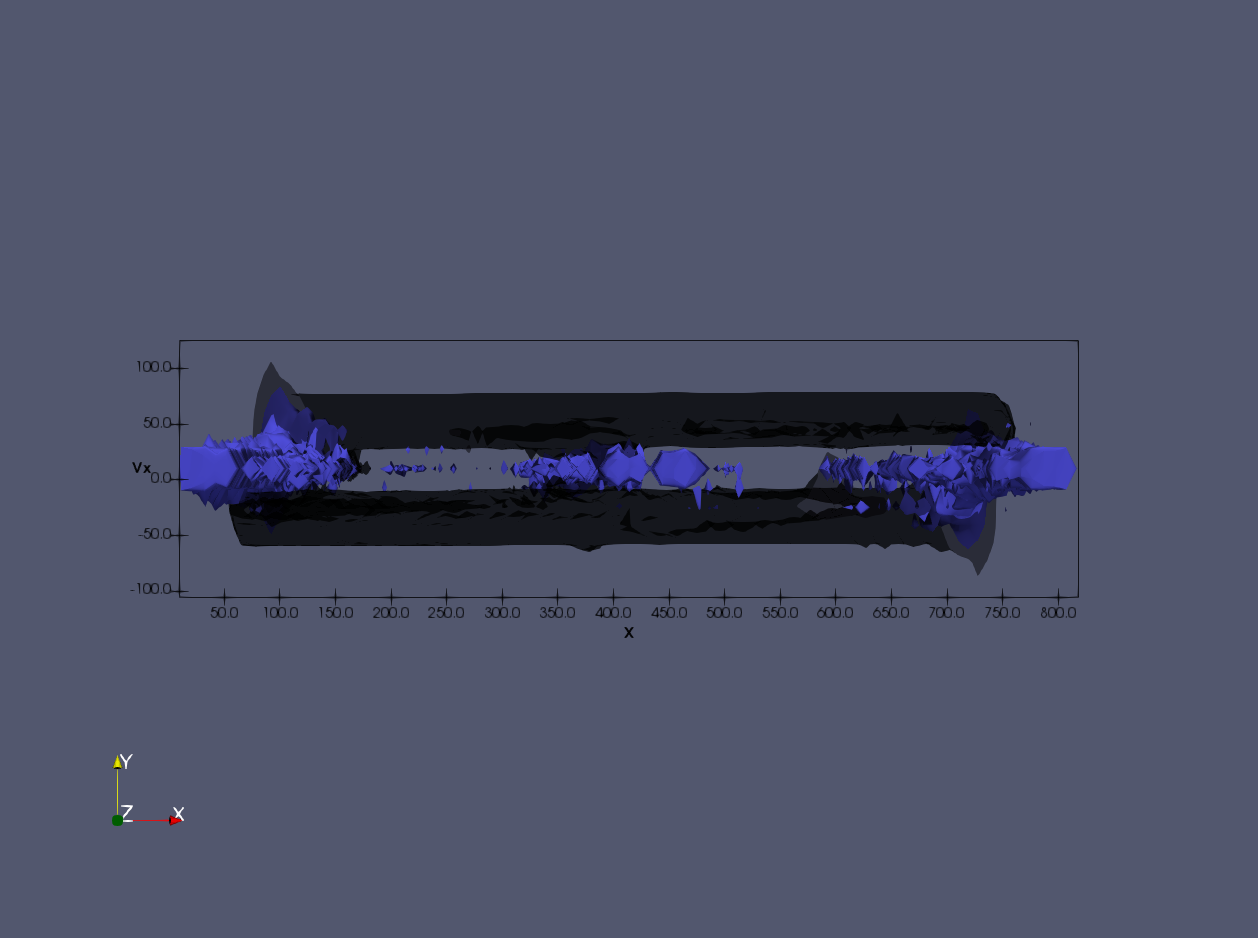
\includegraphics[ width=0.9\textwidth]{fig/3d-hist/trainf10_X_Vx_RealData_and_simD2Q9Q9}
\captionsetup{width=.8\linewidth}
\caption{CAPTION ONE}
\label{fig:comp_RD_D2Q9Q9_1}
\end{minipage}
\begin{minipage}[c]{0.5\linewidth}
\centering
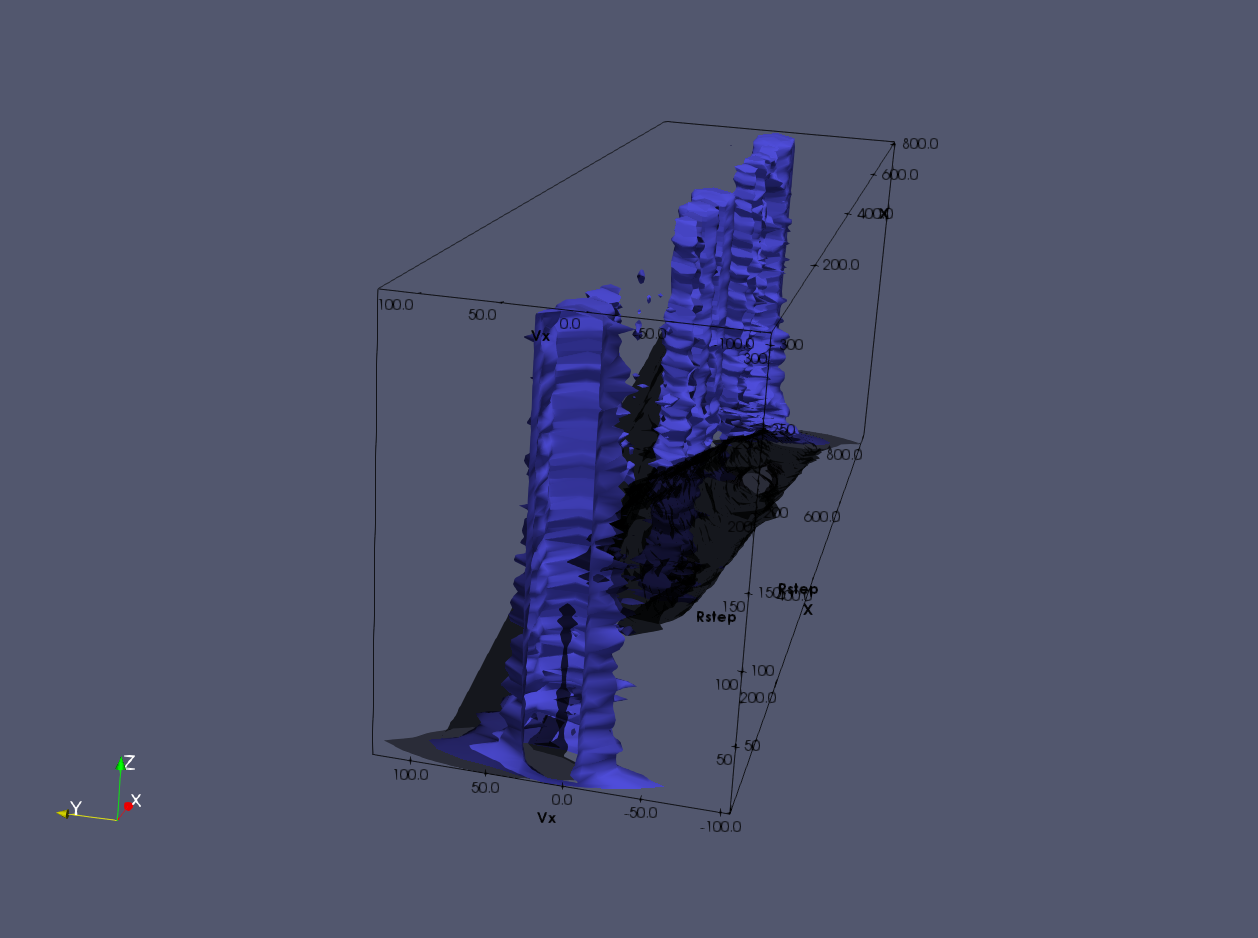
\includegraphics[ width=0.9\textwidth]{fig/3d-hist/trainf10_X_Vx_RealData_and_simD2Q9Q9-2}
\captionsetup{width=.8\linewidth}
\caption{CAPTION TWO}
\label{fig:comp_RD_D2Q9Q9_2}
\end{minipage}
\end{figure}


\FloatBarrier
\subsection{Comparison between RealData and Simulation with TD2Q9 model}

\begin{figure}[ht]
\begin{minipage}[c]{0.5\linewidth}
\centering
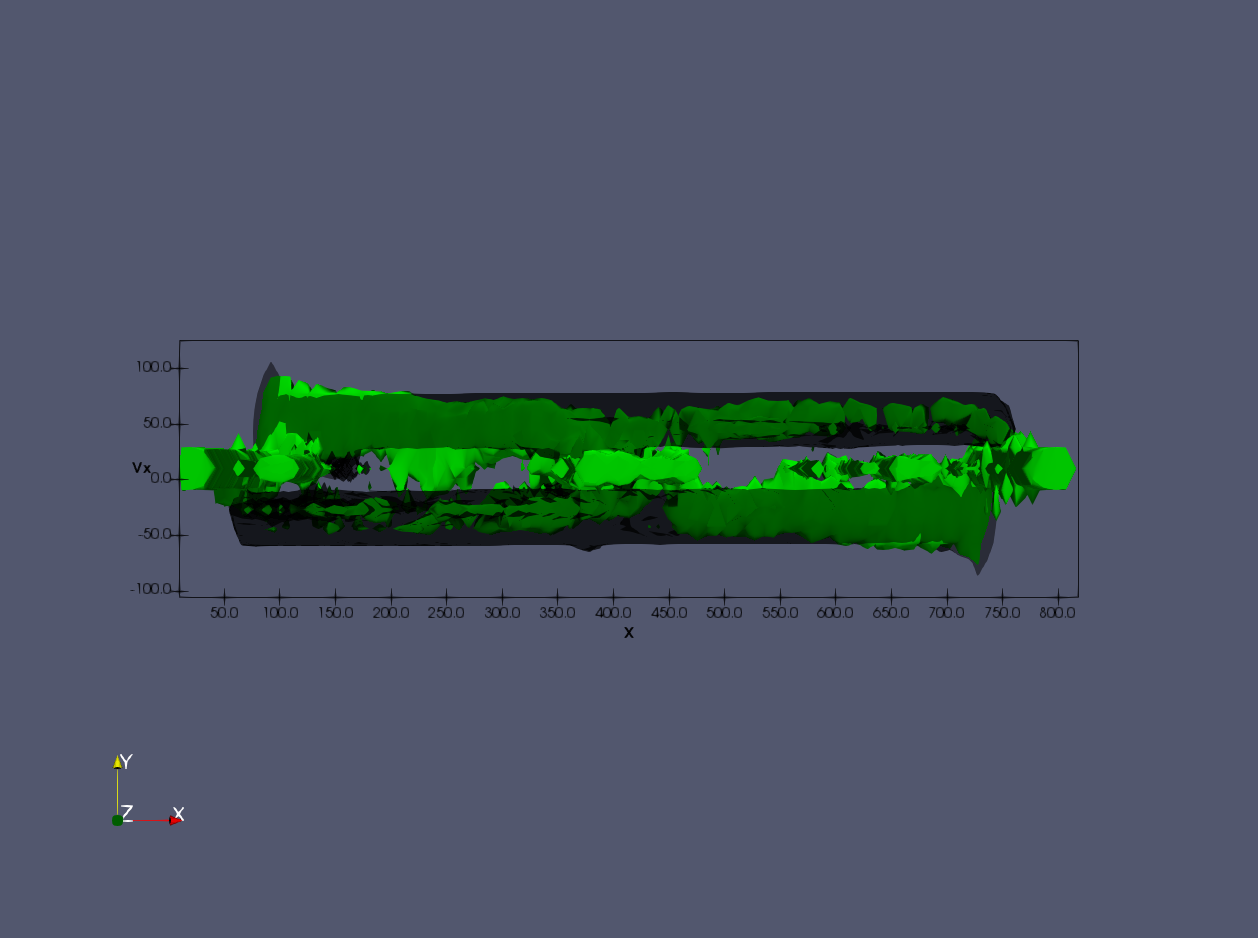
\includegraphics[ width=0.9\textwidth]{fig/3d-hist/trainf10_X_Vx_RealData_and_simTD2Q9}
\captionsetup{width=.8\linewidth}
\caption{CAPTION ONE}
\label{fig:comp_RD_TD2Q9_1}
\end{minipage}
\begin{minipage}[c]{0.5\linewidth}
\centering
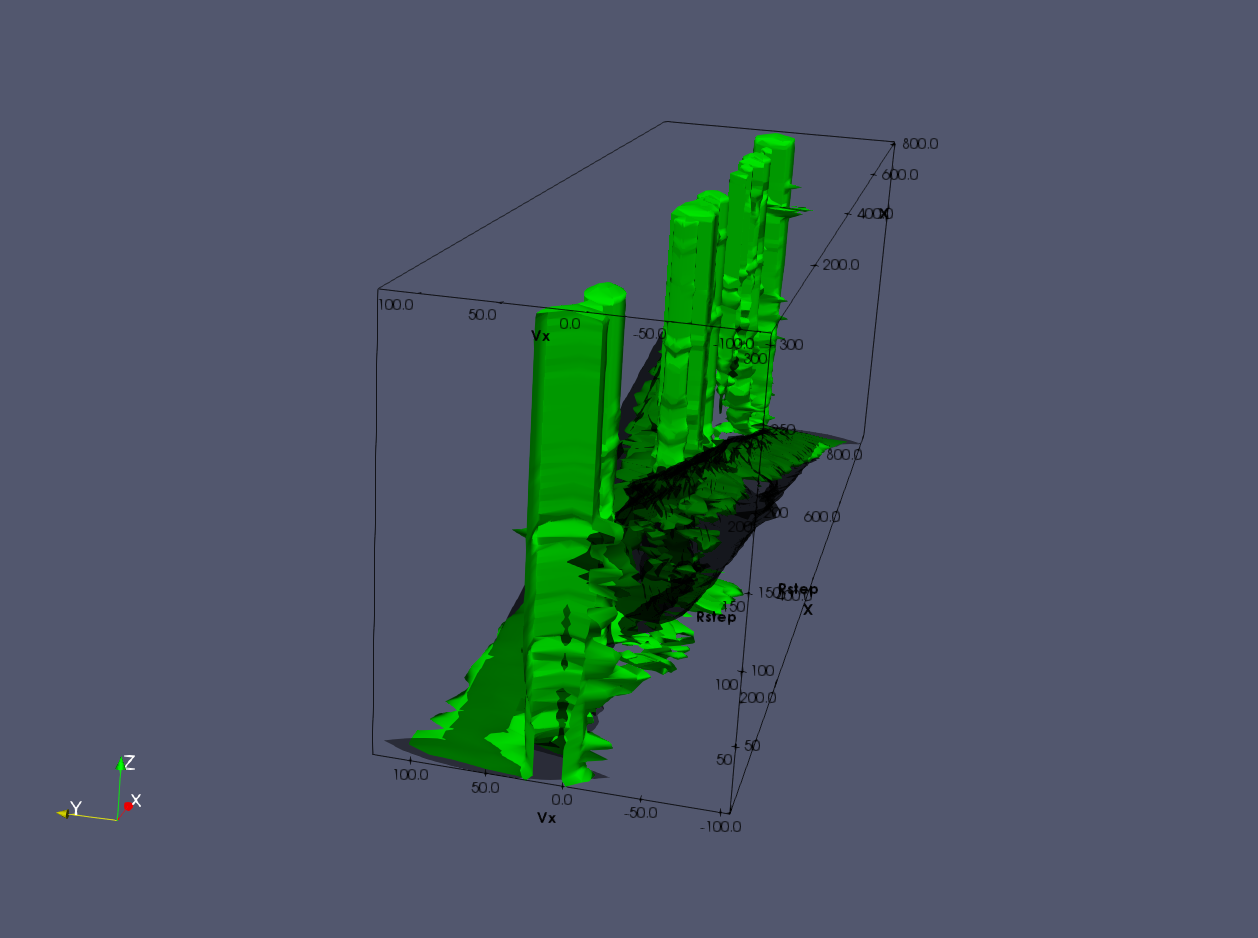
\includegraphics[ width=0.9\textwidth]{fig/3d-hist/trainf10_X_Vx_RealData_and_simTD2Q9-2}
\captionsetup{width=.8\linewidth}
\caption{CAPTION TWO}
\label{fig:comp_RD_TD2Q9_2}
\end{minipage}
\end{figure}


\FloatBarrier
\subsection{Comparison between RealData and Simulation with TD2Q9Q9 model}

\begin{figure}[ht]
\begin{minipage}[c]{0.5\linewidth}
\centering
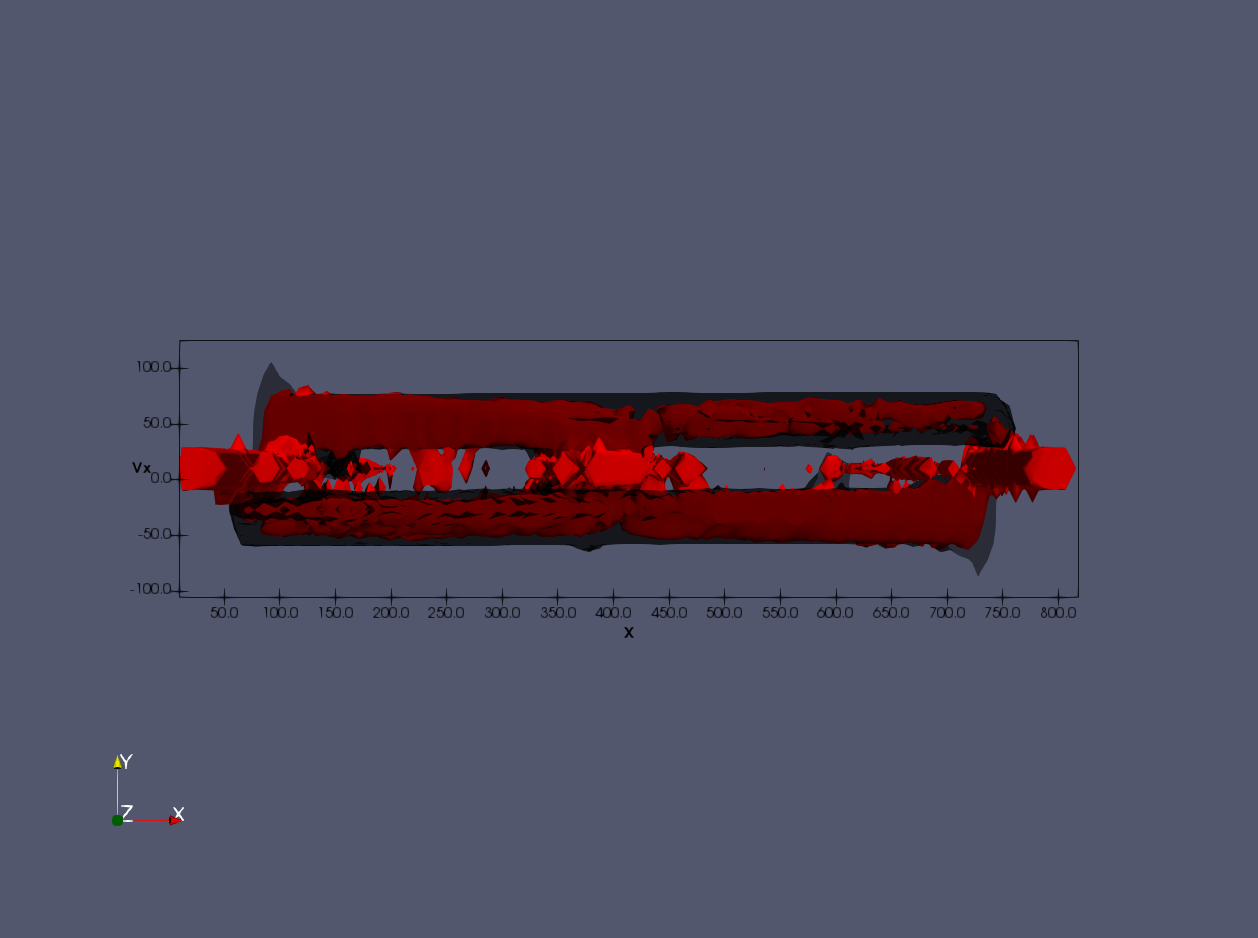
\includegraphics[ width=0.9\textwidth]{fig/3d-hist/trainf10_X_Vx_RealData_and_simTD2Q9Q9}
\captionsetup{width=.8\linewidth}
\caption{CAPTION ONE}
\label{fig:comp_RD_TD2Q9Q9_1}
\end{minipage}
\begin{minipage}[c]{0.5\linewidth}
\centering
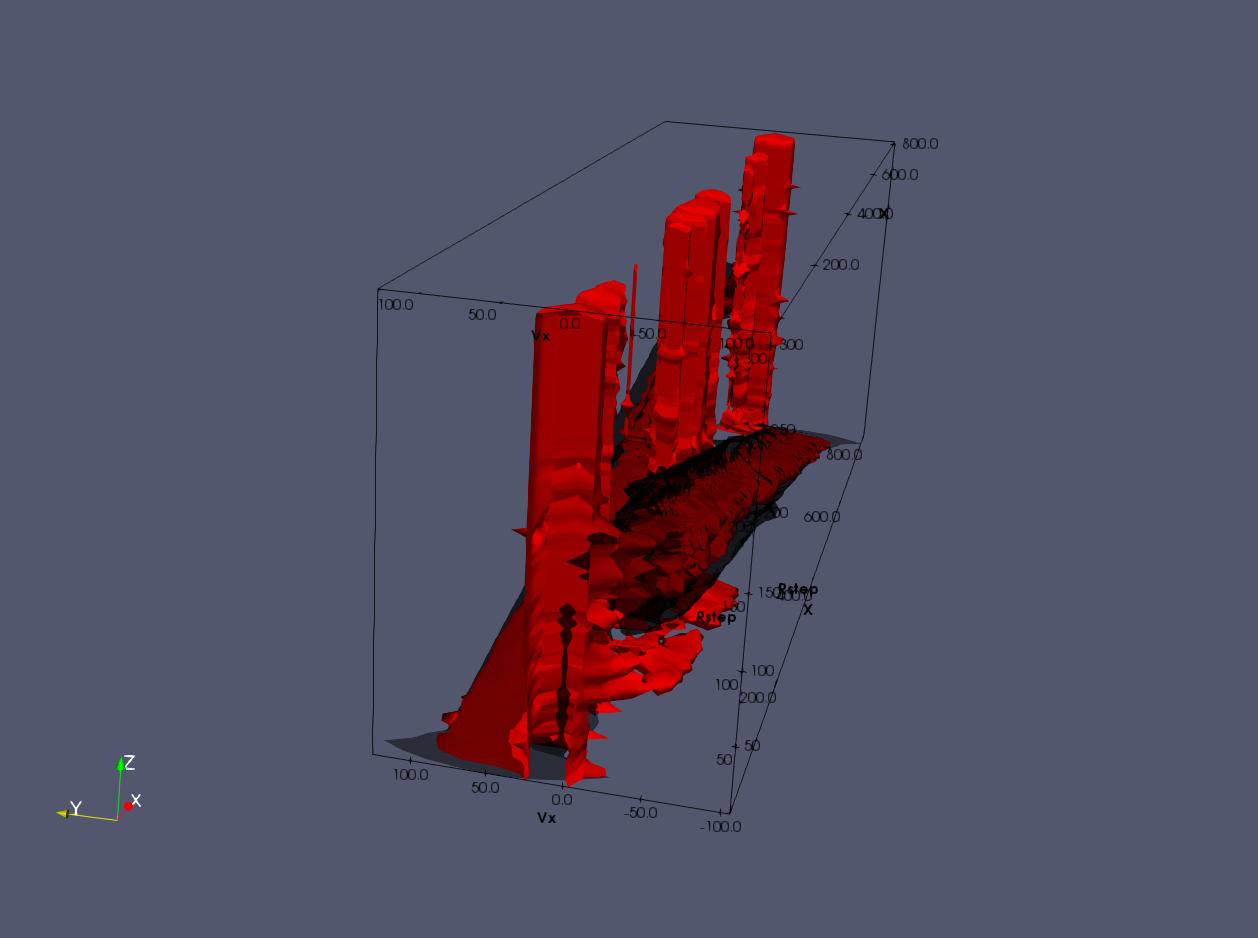
\includegraphics[ width=0.9\textwidth]{fig/3d-hist/trainf10_X_Vx_RealData_and_simTD2Q9Q9-2}
\captionsetup{width=.8\linewidth}
\caption{CAPTION TWO}
\label{fig:comp_RD_TD2Q9Q9_2}
\end{minipage}
\end{figure}


\FloatBarrier
\end{document}
